\section{Problem Statement}

\begin{figure}[h]
    \centering
    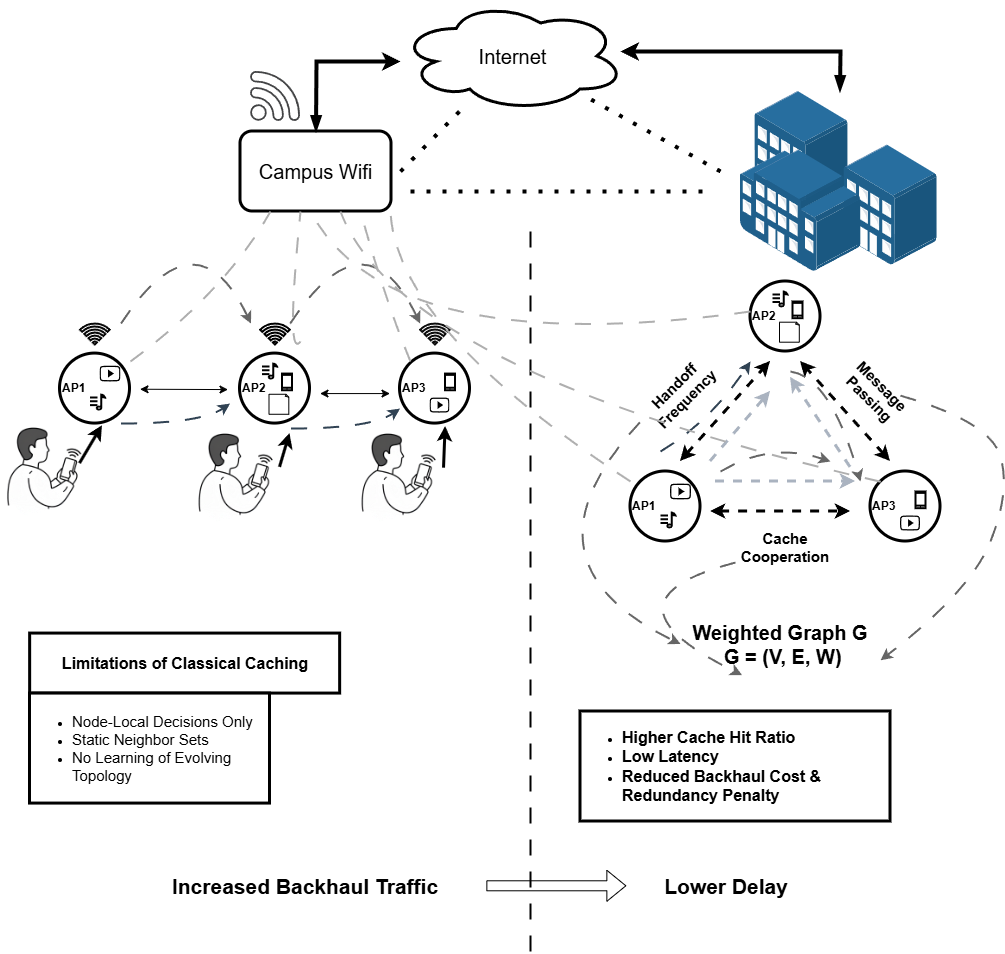
\includegraphics[width=0.8\textwidth]{iot_project.drawio.png}
    \caption{Traditional Caching vs Cooperative Caching}
    \label{fig}
    \vspace{1\baselineskip}
\end{figure}

Edge caching is a key mechanism for reducing latency and backhaul congestion in IoT-driven edge networks. Such systems consist of distributed edge nodes (e.g., access points or gateways) that serve mobile users under limited storage capacity. Due to user mobility and spatial locality, content requests observed at different edge nodes are correlated rather than independent.

In practice, these correlations induce a structured interaction topology among edge nodes. We model the edge network as a weighted graph:

\[
G = (V, E, W),
\]

where $V = \{v_1, \dots, v_N\}$ denotes the set of edge nodes, and $W(i,j)$ quantifies the strength of mobility-induced interaction between nodes $v_i$ and $v_j$, derived from aggregated user handoff patterns.

Each node $v_i$ maintains a cache $\mathcal{K}_i \subseteq \mathcal{C}$ subject to capacity constraint $C_i$. Content requests are generated according to synthetic demand distributions designed to reflect realistic workload characteristics, including global popularity skew and spatial locality across nodes.

Existing caching strategies typically operate in one of two ways:

\begin{itemize}
    \item \textbf{Node-local policies}, which update $\mathcal{K}_i$ based solely on local request history,
    \item \textbf{Heuristic cooperative policies}, which incorporate limited neighbor information using predefined neighborhood structures.
\end{itemize}

However, these approaches do not explicitly leverage the mobility-induced topology $G$ when determining cache placement decisions. As a result, they often lead to redundant content replication, inefficient cache utilization, and increased backhaul traffic.

We therefore define the topology-aware cooperative caching problem as follows:

\textbf{Given:}
\begin{itemize}
    \item A static mobility-derived graph $G$,
    \item Synthetic request streams generated per node,
    \item Cache capacity constraints $\{C_i\}$,
\end{itemize}

\textbf{Find a joint caching policy}

\[
\pi : (G, \{\mathcal{K}_i\}) \rightarrow \{\mathcal{K}_i'\},
\]

that determines cache placement across nodes to maximize overall system utility, measured in terms of:

\begin{itemize}
    \item Cache hit ratio,
    \item Latency reduction,
    \item Backhaul traffic minimization,
    \item Reduction of redundant replication across neighboring nodes.
\end{itemize}

The central research question is whether explicitly incorporating the mobility-derived topology $G$ into the caching policy $\pi$ yields measurable performance improvements over node-local and heuristic cooperative approaches.
